\documentclass{beamer}

\usepackage[polish]{babel}
\usepackage[utf8]{inputenc}
\usepackage[T1]{fontenc}
\usepackage{hyperref}
\usepackage{graphicx}
\usepackage{multicol}
\usepackage{tabularx}
\usepackage{tikz}

\usetikzlibrary{positioning}

\mode<presentation>{\usetheme{Dresden}}
\setbeamercovered{dynamic}

\title{Component-based system for management of multilevel virtualization of networking resources}
\subtitle{System komponentowy wspomagający wielopoziomową wirtualizecję zasobów sieciowych}
\author{Robert Boczek \and Dawid Ciepliński \\ ~ \\ prof. dr hab. inż Krzysztof Zieliński}
\date{29.03.2011}

\begin{document}

\begin{frame}

	\titlepage

\end{frame}

\newcounter{enumi_chapter}

\begin{frame}{Introduction}

	\begin{enumerate}

		\item Introduction \pause

		\item Context

			\begin{enumerate}
			
				\item QoS-aware networking \pause
				\item Resource virtualization approaches \pause
				\item Multilevel network virtualization
					
					\begin{enumerate}
						\item Virtual network resources
						\item Fine-grained QoS control
						\item Virtual appliances
						\item ,,Network in a box'' concept
					\end{enumerate}

					\pause

				\item Applications and benefits of virtual infrastructures

					\begin{enumerate}
						\item Testing and simulations
						\item Improving server-side infrastructure scalability
						\item Infrastructure as a service
						\item The role of resource virtualization in the SOA stack
					\end{enumerate}
			
			\end{enumerate}
	
	\end{enumerate}

\end{frame}

\setcounter{enumi_chapter}{\value{enumi}}

\begin{frame}{Multilevel network virtualization}
		
	\begin{figure}[H]
		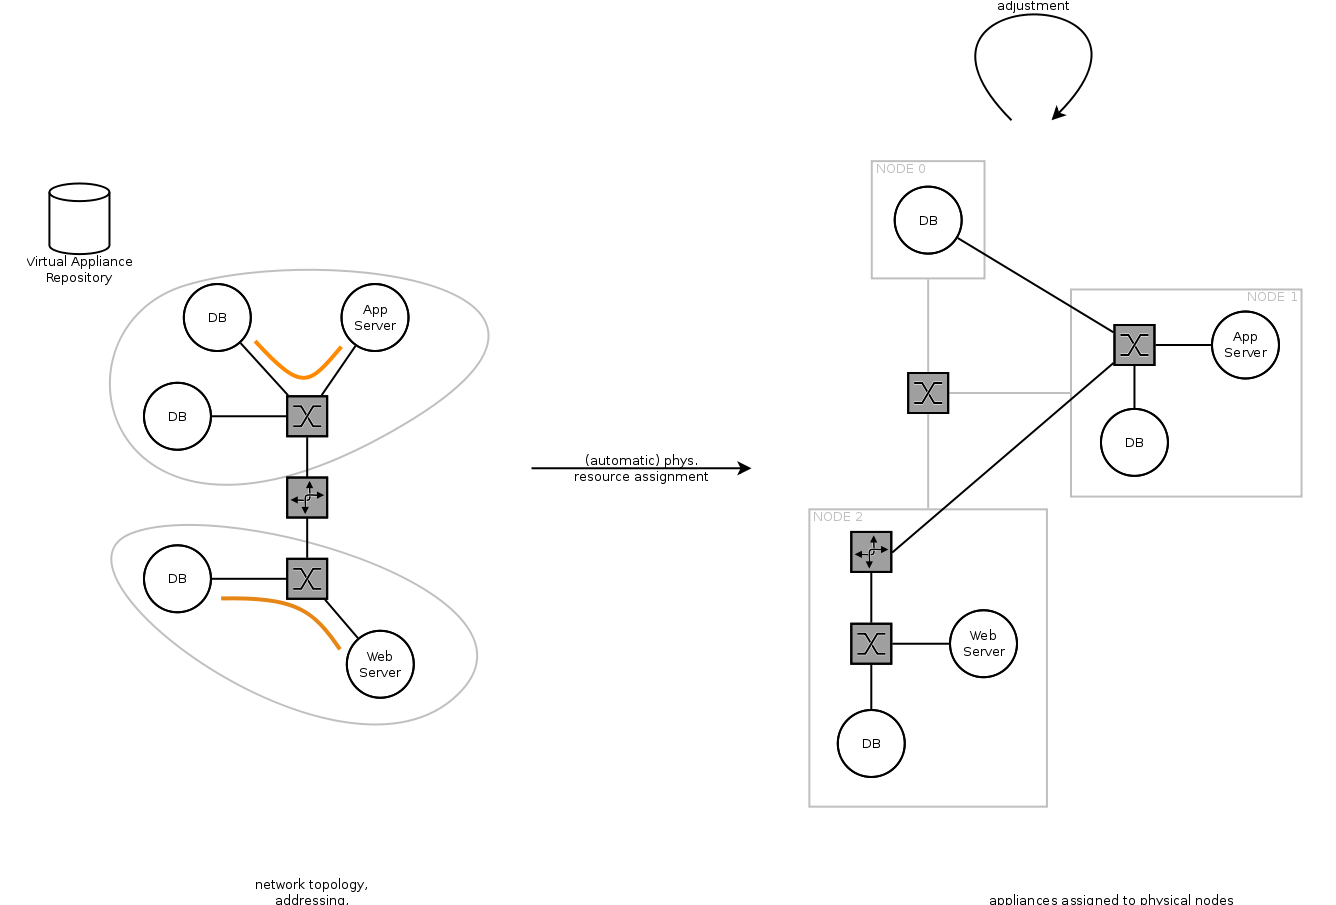
\includegraphics[width=\textwidth]{img/scope.jpg}
	\end{figure}

\end{frame}

\setcounter{enumi_chapter}{\value{enumi}}


\begin{frame}{Requirements analysis}

	\begin{enumerate}
		\setcounter{enumi}{\value{enumi_chapter}}

		\item Requirements analysis

			\begin{enumerate}

				\item Functional requirements

					\begin{enumerate}
						\item Instantiation
						\item Discovery
						\item Accounting
					\end{enumerate}

					\pause
			
			 \item Non-functional requirements \pause

			 \item Underlying environment characteristics \pause
		 
			 \item General approach and problems it imposes

			 	\begin{enumerate}
					\item Load balancing / Deployment
					\item Infrastructure isolation
					\item Broadcast domain preservation
					\item Constraints
				\end{enumerate}
		 
			\end{enumerate}

	\end{enumerate}

\end{frame}

\setcounter{enumi_chapter}{\value{enumi}}


\begin{frame}{Solaris OS as a resource virtualization environment}

	\begin{enumerate}
		\setcounter{enumi}{\value{enumi_chapter}}

		\item Solaris OS as a resource virtualization environment

			\begin{enumerate}
				\item General information
				\item Lightweight OS-level virtualization with Solaris Containers
				\item Crossbow - network virtualization technology
				\item Resource access control
			\end{enumerate}

	\end{enumerate}

\end{frame}

\setcounter{enumi_chapter}{\value{enumi}}


\begin{frame}{The system architecture}

	\begin{enumerate}
		\setcounter{enumi}{\value{enumi_chapter}}

		\item The system architecture

		\begin{enumerate}
			\item High-level design \pause
			\item System components and their responsibilities

				\begin{enumerate}
					\item Assigner
					\item Supervisor
					\item Worker
				\end{enumerate}

				\pause
			
			\item Crossbow resources instrumentation \pause
			\item Domain model and data flows
		\end{enumerate}

	\end{enumerate}

\end{frame}

\setcounter{enumi_chapter}{\value{enumi}}

\begin{frame}{Gui console}
		
	\begin{figure}[H]
		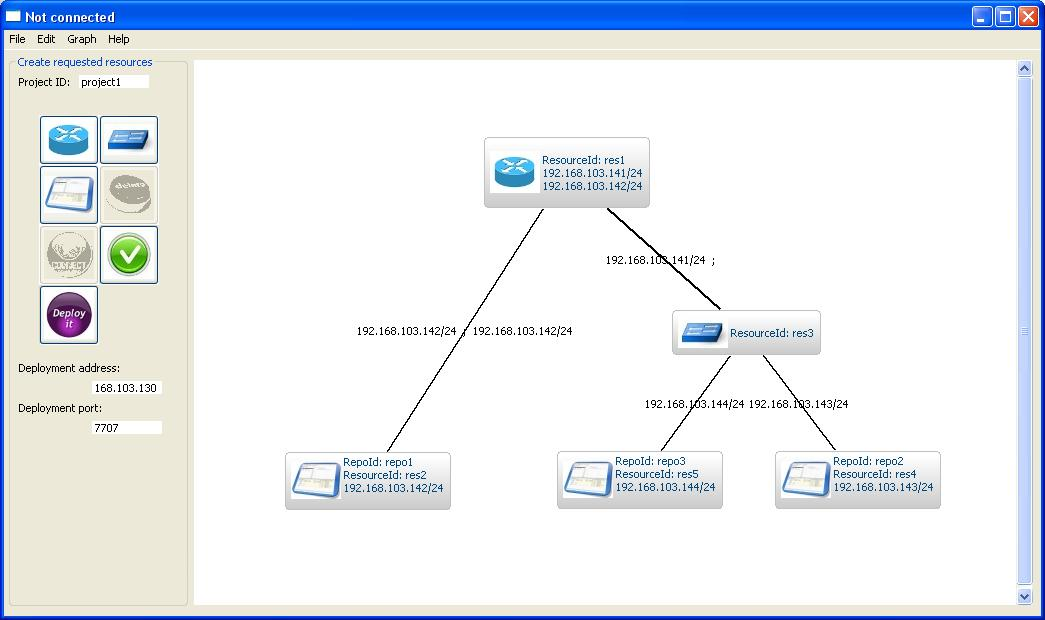
\includegraphics[width=\textwidth]{img/network.jpg}
	\end{figure}

\end{frame}

\setcounter{enumi_chapter}{\value{enumi}}


\begin{frame}{Implementation}

	\begin{enumerate}
		\setcounter{enumi}{\value{enumi_chapter}}

	\item Implementation

		\begin{enumerate}
			\item Implementation environment
			\item Domain model transformation details
			\item Low-level functions access
			\item Building and running the platform
		\end{enumerate}

	\end{enumerate}

\end{frame}

\setcounter{enumi_chapter}{\value{enumi}}


\begin{frame}{Proposals of Case Studies}

	\begin{enumerate}
		\setcounter{enumi}{\value{enumi_chapter}}

		\item Clustered GlassFish
		\item Multimedia server

 %    \section{Clustered GlassFish
 %      \subsection{Scenario description
 %      \subsection{GlassFish cluster integration
 %
 %
 %    \section{Multimedia server
 %      \subsection{Scenario description
 %      \subsection{Resource access requirements
 %      \subsection{Providing tunable and scalable virtual infrastructure
	
	\end{enumerate}

\end{frame}

\setcounter{enumi_chapter}{\value{enumi}}


\begin{frame}{Summary}

	\begin{enumerate}
		\setcounter{enumi}{\value{enumi_chapter}}

		\item Summary

			\begin{enumerate}
				\item Conclusions
				\item Achieved goals
				\item Further work
			\end{enumerate}

	\end{enumerate}

\end{frame}

\setcounter{enumi_chapter}{\value{enumi}}

\end{document}

